\documentclass[12pt]{book}
\usepackage{a4wide}
\usepackage{fancyhdr}
\usepackage{makeidx}
\usepackage{tabularx}
\usepackage{epsfig}
\usepackage{amssymb}
\usepackage{amsmath}
\usepackage{epic}
\usepackage{eepic}
\usepackage{ecltree}
\usepackage{rotating}
\usepackage{color}
\usepackage[french]{babel}
\usepackage[latin1]{inputenc}
\usepackage[OT1]{fontenc}
\usepackage{hevea}
\def\arbreun#1#2{
\begin{bundle}{#1}
    \chunk{#2}
\end{bundle}
}
\def\arbrebin#1#2#3{
\begin{bundle}{#1}
    \chunk{#2}
    \chunk{#3}
\end{bundle}
}
\def\arbretern#1#2#3#4{
\begin{bundle}{#1}
    \chunk{#2}
    \chunk{#3}
    \chunk{#4}
\end{bundle}
}
\def\cleardoublepage{\clearpage\if@twoside \ifodd\c@page\else
\hbox{}\thispagestyle{empty}\newpage\if@twocolumn\hbox{}\newpage\fi\fi\fi}
\renewcommand{\chaptermark}[1]{\markboth{#1}{}}
\renewcommand{\sectionmark}[1]{\markright{#1}}
\definecolor{part}{rgb}{0.7, 0.7, 1}\definecolor{chapter}{rgb}{0.8, 0.8, 1}\definecolor{section}{rgb}{0.9, 0.9, 1}\definecolor{subsection}{rgb}{0.95, 0.95, 1}\definecolor{subsubsection}{rgb}{0.97, 0.97, 1}\pagestyle{empty}
\begin{document}
    \epsfig{figure=cube.eps,width=.7\columnwidth}

\clearpage% page: 0
    \begin{tabular}[c]{|c|}
      \hline
      \textbf{Clients} \\ \hline
      NumClient\\
      Ville\\
      �ge\\
      Sexe\\ \hline
    \end{tabular}
    \begin{picture}(25,35)(0,0)
      \put(0,18){\line(5,-1){30}}
    \end{picture}
    \ \begin{tabular}[c]{|c|}
      \hline
      \textbf{Ventes} \\ \hline
      RefClient\\
      RefTemps\\
      RefProduit\\
      Montant\\ \hline
    \end{tabular}
    \raisebox{-70pt}{\begin{picture}(25,140)(0,0)
        \put(0,50){\line(3,-2){30}}
        \put(0,70){\line(1,2){30}}
      \end{picture}}
    \begin{tabular}[c]{l}
      \begin{tabular}[t]{|c|}
        \hline
        \textbf{Temps} \\ \hline
        NumTemps\\
        Tranche Horaire\\
        Mois\\
        Jour\\
        Ann�e\\
        \hline
      \end{tabular}\\
      \begin{tabular}[t]{|c|}
        \hline
        \textbf{Produit} \\ \hline
        NumProduit\\
        Cat�gorie\\
        Classe de Prix\\
        Couleur\\ \hline
      \end{tabular}
    \end{tabular}

\clearpage% page: 1
    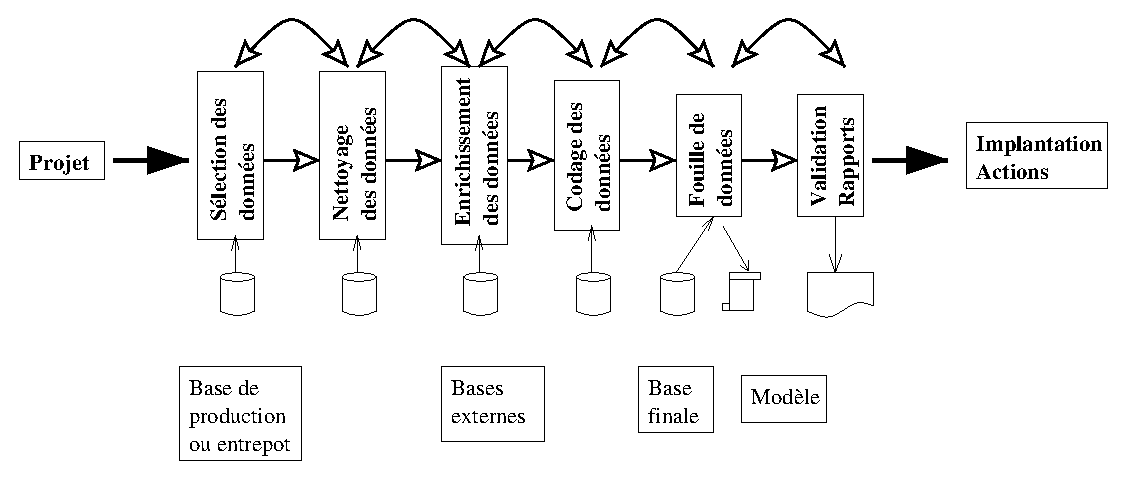
\epsfig{file=kdd.eps,width=\textwidth}

\clearpage% page: 2
    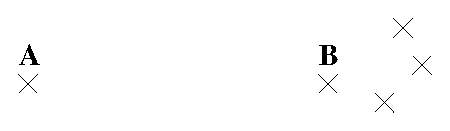
\epsfig{file=ppvoisins.eps}

\clearpage% page: 3
    \setlength{\GapWidth}{10pt}
    \arbrebin {\fbox{\texttt{MS > 5000}}} 
        {Y}
        {\arbrebin {\fbox{\texttt{age > 25}}}  
           {\setlength{\GapWidth}{80pt}
            \arbrebin {\fbox{\texttt{autres comptes}}} {Y} {N}}  
           {N}
        }  
     \setlength{\GapWidth}{4pt}   

\clearpage% page: 4
          \input{perceptron.pstex_t}

\clearpage% page: 5
             \epsfig{file=sigma.eps,height=4cm,width=8cm}

\clearpage% page: 6
          \input{pmc.pstex_t}

\clearpage% page: 7
          \input{pmc41.pstex_t}

\clearpage% page: 8
\newcommand{\monlabel}[1]{\mbox{\bfseries\textsf{#1}}\dotfill}
\newenvironment{monglossaire}%
{\begin{list}{}%
    {\renewcommand{\makelabel}{\monlabel}%
      \setlength{\labelwidth}{.3\columnwidth}%
      \setlength{\itemsep}{3cm}%
%      \setlength{\parsep}{140pt}%
      \setlength{\labelsep}{0pt}%
      \setlength{\leftmargin}{\labelwidth}
      \addtolength{\leftmargin}{\labelsep}%
    }%
}%
{\end{list}}
\end{document}
